% Options for packages loaded elsewhere
\begin{document}

\hypertarget{exclusion-criteria}{%
\subsection{Exclusion criteria}\label{exclusion-criteria}}

\begin{table*}

\caption{\label{tab:descTable}\label{descTable}Descriptive statistics for the DVs broken down
                     by experimental condition.}
\centering
\begin{tabular}[t]{llrrrrrr}
\toprule
Measure & Condition & $n$ & $M$ & $SE_M$ & $SD$ & min & max\\
\midrule
 & Content, feedback & 41 & 13.22 & 0.508 & 3.25 & 2 & 19\\

 & Content, no feedback & 42 & 12.79 & 0.465 & 3.02 & 7 & 19\\

 & General, feedback & 40 & 10.97 & 0.533 & 3.37 & 1 & 17\\

 & General, no feedback & 40 & 10.47 & 0.449 & 2.84 & 5 & 16\\

\multirow{-5}{*}{\raggedright\arraybackslash Total correct} & Rereading & 40 & 10.88 & 0.443 & 2.80 & 4 & 17\\
\cmidrule{1-8}
 & Content, feedback & 41 & 3.15 & 0.258 & 1.65 & 0 & 7\\

 & Content, no feedback & 42 & 3.38 & 0.257 & 1.67 & 0 & 7\\

 & General, feedback & 40 & 4.17 & 0.318 & 2.01 & 0 & 8\\

 & General, no feedback & 40 & 4.58 & 0.288 & 1.82 & 1 & 9\\

\multirow{-5}{*}{\raggedright\arraybackslash Total intrusors} & Rereading & 40 & 4.62 & 0.350 & 2.21 & 1 & 10\\
\bottomrule
\end{tabular}
\end{table*}

Prior to analysing the data, we excluded participants based on a priori
set criteria. Participants who spent less than or equal to 90 seconds on
the practice text were excluded (1 exclusion). Further, we wanted to
exclude participants who had no correct answers on the final test (0
exclusions). Finally, we excluded participants who had stated that they
had reading deficits (3 exclusions). This left us with a total sample of
203 participants. The descriptives for the sample are shown in Table
\ref{descTable}.

\begin{figure}
\centering
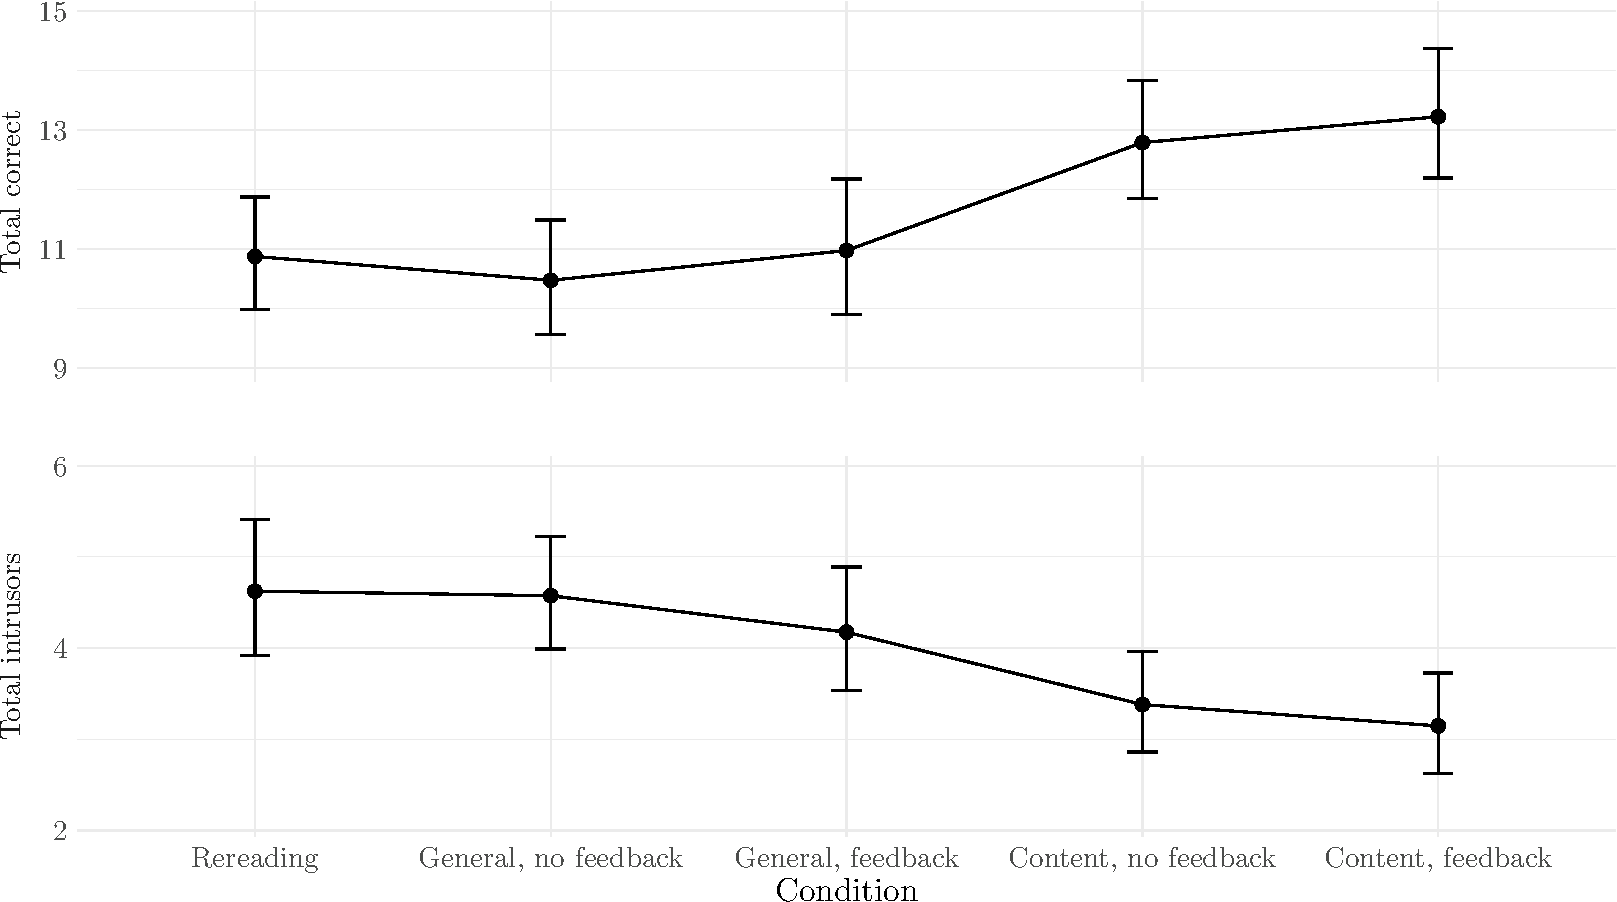
\includegraphics{../analyses/images/descFig-1.pdf}
\caption{Mean number of correct answers and mean number of intrusive
distractors chosen, broken down by experimental condition. Error bars
show the 95\% confidence intervals around the means.}
\end{figure}

\hypertarget{interpolated-activity-effect}{%
\subsection{Interpolated activity
effect}\label{interpolated-activity-effect}}

Our first two hypotheses are concerned with the effects of different
interpolated activities on the total number of correct answers and total
number of intrusive distractors chosen. To test these hypotheses, we
focused only on the groups which did not receive feedback (\(n\) = 122).
This was done because there was no feedback option for the rereading
group, and we did not want to treat the feedback and no-feedback
general-knowledge and content-related testing groups as equivalent
without strong evidence supporting that assumption.

The correlation between our DVs calculated on the whole sample is
\(r(201) =\) -.707 (95\% CI: {[}-.77, -.63{]}, \(p\) \textless{} .0001).
Given this fact, we ran a one-way MANOVA with interpolated activity as the 
independent variable and the total number of correct and intrusive options 
chosen as dependent variables. Conducting a MANOVA guards against an 
inflation of Type 1 errors that running multiple ANOVAs on highly correlated 
dependent variables is prone to
\citep{tabachnickUsingMultivariateStatistics2012, 
fieldDiscoveringStatisticsUsing2012}
Further, running a single MANOVA increases the chance of discovering effects 
of different treatments \citep{tabachnickUsingMultivariateStatistics2012}.

A power analysis conducted prior to analyzing the data
\citep[using the G*Power software by][]{faulStatisticalPowerAnalyses2009}
has shown that we should have above 80\% power to detect effects which
fall between small and medium (Cohen's \(f^2\ \gtrsim 0.06\)), at an
\(\alpha\) level of .025, with a sample size of 110 participants. Note
that larger effects are expected based on prior studies.

Pillai's V for the analysis is .126, \(p = .004\) (Wilks' \(\Lambda\) =
.875, \(p = .003\)). The effect size, calculated as
\(\omega^2_{mult} = .109\) (bootstrap
median\footnote{All bootstrap estimates taken from 10000 replications.}
= .132, \(BC_\alpha\) 95\% CI = {[}.011, .202{]})\footnote{
Cohen's \(f^2 = 0.051\) (calculated according to Equation 12 in
\citealp{steynjrEstimatingEffectSize2009}).
}. To further inspect the relationship of the interpolated activities
with our dependent variables, we conducted a Roy-Bargmann stepdown
analysis, as suggested by
\citeauthor{tabachnickUsingMultivariateStatistics2012}
(\citeyear{tabachnickUsingMultivariateStatistics2012}; a linear
discriminant analysis with the same aim is available in the
supplementary materials). According to
\citet{tabachnickUsingMultivariateStatistics2012}, the higher priority
variable can be chosen based on theoretical or practical grounds. Since
the total number of correct answers is the criterion that determines a
student's success in a testing context, we chose this dependent variable
as the higher priority one. We first conducted an ANOVA with interpolated 
activity type as the independent variable and the total number of correct 
answers as the dependent variable.

As could be expected, the ANOVA points to a differential effect of our
conditions on the total number of correct answers, with \(F(2, 119)\) =
7.541, \(p = .001\). Following the ANOVA, we conducted an ANCOVA, with
the total number of correct answers as the covariate, and the total
number of intrusors as the dependent variable. The results imply a main
effect of the total number of correct answers (\(F(1, 118)\) = 79.674,
\(p < .0001\)), but after controlling for the number of correct
answers, we found no evidence for an effect of interpolated activity
type on the total number of chosen intrusors (\(F (2, 118)\) = 0.844,
\(p = .433\)).

In order to test our first hypothesis, we contrasted (i) the rereading
group with the two test groups, and (ii) the two test groups with each
other, taking only the total number of correct answers as the DV. The
first contrast found no evidence of a difference between the rereading
group and the two test groups (\(t(119)\) = 1.355, \(p = .178\), \(g_s\)
= 0.19, 95\% CI = {[}-0.19, 0.57{]}, Cohen's \(U_{3, g_s}\) = 57.6\%,
probability of superiority = 55.39\%). Therefore, we cannot conclude
that being in the rereading condition, as opposed to being in one of the
two test groups, leads to different learning outcomes. However, there
was a difference between the two test groups (\(t(119)\) = 3.62,
\(p = .0004\), \(g_s\) = 0.66, 95\% CI = {[}0.21, 1.1{]}, Cohen's
\(U_{3, g_s}\) = 74.43\%, probability of superiority = 67.88\%).
Subjects in the content-related-test condition score higher on the final
test than those in the general-knowledge-test condition. These two
findings are not in line with our predictions.

\hypertarget{the-interaction-between-feedback-and-interpolated-activity-type}{%
\subsection{The interaction between feedback and interpolated activity
type}\label{the-interaction-between-feedback-and-interpolated-activity-type}}

The remaining hypotheses deal with the effect of feedback on the total
number of correct answers and the total number of intrusors. Therefore,
these analyses were carried out on the data from participants in the
general and content related test conditions only (\(n\) = 163). To test
these hypotheses, we first conducted a two-way MANOVA with interpolated
activity and feedback as independent variables, and total number of
correct answers and total number of intrusors as the dependent
variables. Again, a power analysis conducted before analysing the data
has shown that we should have above 80\% power to detect effects which
fall between small and medium (Cohen's \(f^2\ \gtrsim 0.05\)), at an
\(\alpha\) level of .025, with a sample size of 145 participants.

Pillai's V for the interpolated activity effect (calculated with type
III sums of squares) is .071, \(p = .003\) (Wilks' \(\Lambda\) = .929,
\(p = .003\)) confirming the main effect of interpolated activity type.
The effect size \(\omega^2_{mult}\) = .065 (bootstrap median = .072,
\(BC_\alpha\) 95\% CI = {[}.008, .140{]})\footnote{
Cohen's \(f^2 = 0.063\), using Equation 12 from
\citet{steynjrEstimatingEffectSize2009}.
}. On the other hand, we found no evidence for an effect of giving feedback
on the linear combination of our two dependent variables --- Pillai's V
= .003, \(p = .800\) (Wilks' \(\Lambda\) = .997, \(p = .800\)). The
estimated effect size is \(\omega^2_{mult}\) = 0. Furthermore, we found no 
evidence for an interaction effect between activity type and feedback --- 
Pillai's V = .001, \(p = .941\) (Wilks' \(\Lambda\) = .999, \(p = .941\)). 
The estimated effect size
\(\omega^2_{mult}\) = 0.

Again, we conducted a follow-up Roy-Bargmann stepdown analysis. In the
ANOVA model with the total number of correct answers as the dependent
variable and the type of interpolated activity, feedback and their
interaction as predictors, only the type of activity seems to be
relevant (\(F(1, 159) = 11.2, p = .001\)). This result also shows that
subjects in the content-related-test condition score higher on the final
test than those in the general-knowledge-test condition, which should
be no surprise given the results of the first stepdown analysis. In the
second step, we fit an ANCOVA model with the total number of correct
answers as the covariate. In this model, the type of interpolated
activity ceases to be a relevant predictor
(\(F(1, 155) = 0.175, p = .676\)). Therefore, we find no evidence for an
effect of the type of interpolated activity nor of feedback on the
number of intrusive distractors chosen. The full models are shown in
Table \ref{rb2-table}.

To summarise, contrary to our expectations, we find no evidence of an
effect of feedback on the total number of correctly answered questions.
Also, we found no evidence for an interaction effect of feedback and
type of interpolated activity on the total number of correct answers.
The same findings apply to the predictions regarding the total number of
intrusors chosen.

\begin{table*}

\caption{\label{tab:rb2Table}\label{rb2-table}ANOVA and ANCOVA models for the second Roy-Bargmann
                     procedure.}
\centering
\begin{tabular}[t]{lrrrr}
\toprule
Term & $SS$ & $df$ & $F$ & $p$\\
\midrule
\addlinespace[0.3em]
\multicolumn{5}{l}{\textbf{ANOVA}}\\
\hspace{1em}Activity & 109.393 & 1 & 11.200 & .001\\
\hspace{1em}Feedback & 3.904 & 1 & 0.400 & .528\\
\hspace{1em}Activity x Feedback & 0.045 & 1 & 0.005 & .946\\
\hspace{1em}Residuals & 1553.046 & 159 &  & \\
\addlinespace[0.3em]
\multicolumn{5}{l}{\textbf{ANCOVA}}\\
\hspace{1em}Activity & 0.301 & 1 & 0.175 & .676\\
\hspace{1em}Feedback & 0.173 & 1 & 0.100 & .752\\
\hspace{1em}Total correct & 63.216 & 1 & 36.760 & < .0001\\
\hspace{1em}Activity x Feedback & 0.813 & 1 & 0.473 & .493\\
\hspace{1em}Activity x Total correct & 0.862 & 1 & 0.501 & .480\\
\hspace{1em}Feedback x Total correct & 0.130 & 1 & 0.075 & .784\\
\hspace{1em}Activity x Feedback x Total correct & 1.229 & 1 & 0.715 & .399\\
\hspace{1em}Residuals & 266.551 & 155 &  & \\
\bottomrule
\end{tabular}
\end{table*}

\hypertarget{constraints-on-generality}{%
\subsection{Constraints on generality}\label{constraints-on-generality}}

\begin{itemize}
\tightlist
\item
  problemi

  \begin{itemize}
  \tightlist
  \item
    samo jedan tip materijala
  \item
    samo studenti
  \end{itemize}
\item
  nisu problemi

  \begin{itemize}
  \tightlist
  \item
    generalizacija na situacije u kojima učenici trebaju savladati
    gradivo koje im je većinom nepoznato
  \item
    nemamo konkretan razlog za vjerovati da bi sadržaj materijala imao
    ikakvog relevantnog efekta, odnosno da se efekt ne bi javio s drugim
    sadržajem
  \end{itemize}
\end{itemize}

\hypertarget{deviations-from-the-preregistered-analysis-plan}{%
\subsection{Deviations from the preregistered analysis
plan}\label{deviations-from-the-preregistered-analysis-plan}}

Initially, we had planned to do a robustness check of our findings using
data with an additional exclusion criterion, based on the number of
times each participant had read each of the three parts of the main
text. This analysis was never conducted because (i) applying this
criterion would have lead to unacceptably low power and (ii) the
participants' estimates of the number of times they had read each part
were similarly distributed across all conditions. Further, we had
planned to conduct a TOST procedure to test whether there is no
difference between the content-related and general-knowledge testing
groups. This analysis was not conducted because we did find a
difference. A Bayesian t-test was also considered for the same
comparison, but was dropped early on due to some conceptual concerns.

\end{document}
